\documentclass[conference]{IEEEtran}
\IEEEoverridecommandlockouts
% The preceding line is only needed to identify funding in the first footnote. If that is unneeded, please comment it out.
\usepackage{cite}
\usepackage{amsmath,amssymb,amsfonts}
\usepackage{algorithmic}
\usepackage{graphicx}
\usepackage{textcomp}
\usepackage{xcolor}
\usepackage[brazilian]{babel}
\usepackage[utf8]{inputenc}
\usepackage[T1]{fontenc}
\usepackage{listings}
\usepackage{color}
\usepackage{float}
\usepackage{multirow}

\definecolor{dkgreen}{rgb}{0,0.6,0}
\definecolor{gray}{rgb}{0.5,0.5,0.5}
\definecolor{mauve}{rgb}{0.58,0,0.82}

\lstset{frame=tb,
  language=Java,
  aboveskip=3mm,
  belowskip=3mm,
  showstringspaces=false,
  columns=flexible,
  basicstyle={\small\ttfamily},
  numbers=none,
  numberstyle=\tiny\color{gray},
  keywordstyle=\color{blue},
  commentstyle=\color{dkgreen},
  stringstyle=\color{mauve},
  breaklines=true,
  breakatwhitespace=true,
  tabsize=3
}
\lstset{language=Python}
\def\BibTeX{{\rm B\kern-.05em{\sc i\kern-.025em b}\kern-.08em
    T\kern-.1667em\lower.7ex\hbox{E}\kern-.125emX}}
\begin{document}

\title{Relatório do Laboratório 5: \\ Estratégias Evolutivas\\
}

\author{\IEEEauthorblockN{Isabelle Ferreira de Oliveira}
\IEEEauthorblockA{\textit{CT-213 - Engenharia da Computação 2020} \\
\textit{Instituto Tecnológico de Aeronáutica (ITA)}\\
São José dos Campos, Brasil \\
isabelle.ferreira3000@gmail.com}
}

\maketitle

\begin{abstract}
Esse relatório documenta a implementação de uma estratégia evolutiva simples e comparação de seu desempenho com o de CMA-ES em funções usadas como \textit{benchmark} para algoritmos de otimização. Essas funções utilizadas eram uma esfera transladada, e as fuções de Ackley, Schaffer 2 e Rastrigin 2D.
\end{abstract}

\begin{IEEEkeywords}
Estratégias evolutivas, CMA-ES, \textit{benchmark}, Ackley, Schaffer 2, Rastrigin 2D
\end{IEEEkeywords}

\section{Introdução}
Otimização consiste em encontrar o mínimo (ou máximo) de uma função, ou seja, encontrar o conjunto de parâmetros que levem essa função ao seu mínimo (ou máximo). Também pode ser visto como encontrar a melhor solução dentre todas as soluções viáveis. Nesses problemas de otimização também é possível haver restrições acerca dos parâmetros que serão analisados.

Dentre os mais diversos tipos de algoritmos de otimização, existem os métodos baseado em população. Esses métodos mantêm uma população de possíveis soluções, a fim de tentar encontrar diferentes mínimos locais da função a ser analisada, melhorando assim as chances de se obter uma solução promissora. Um exemplo famoso de algoritmo de otimização baseado em população é o \textit{Particle Swarm Optimization} (PSO).

O pseudo-código desse algoritmo para maximização pode ser visto na subseção a seguir. Em seguida, será apresentado como esse algoritmo foi implementado no contexto do laboratório.

\subsection{Particle Swarm Optimization (PSO)}
Será considerado uma classe \textit{ParticleSwarmOptimization}, representando o algoritmo PSO. Além disso, o pseudocódigo do uso do algoritmo a partir dessa classe é o mostrado a seguir. Nesse pseudocódigo, \textit{pso} é o objeto da classe \textit{ParticleSwarmOptimization}.

\begin{lstlisting}
for i in range(num_evaluations):
	position = pso.get_position_to_evaluate()
	value = quality_function(position)
	pso.notify_evaluation(value)
\end{lstlisting}

No pseudocódigo acima, \textit{quality\underline{\space}function()} é a função a ser maximizada. Assim, iterativamente por tantas vezes até se atingir uma convergência satisfatória ao(à) programador(a), o algoritmo calculará o valor da função para cada partícula na população de candidatas à solução. Para cada partícula, então, após esse cálculo, a função \textit{notify\underline{\space}evaluation()} compara o resultado obtido aos obtidos anteriormente a fim de encontrar o valor maximizado. Uma ideia de implementação em pseudocódigo da função \textit{notify\underline{\space}evaluation()} foi apresentada a seguir.

\begin{lstlisting}
def notify_evaluation(value):
	current_particle = get_current_particle_to_evaluate()

	if value > current_particle.my_best_value:
		current_particle.my_best_value = value
		current_particle.my_best_position = current_particle.position

	if value > global_best_value:
		global_best_value = value
		global_best_position = current_particle.position

	num_particle_evaluated = num_particle_evaluated + 1
	if num_particle_evaluated == num_particles:
		num_particle_evaluated = 0
		advance_generation()
\end{lstlisting}

A função \textit{advance\underline{\space}generation()} é a responsável por atualizar os valores de cada partícula a cada geração de população. As posições de cada particula são acrescidas de uma velocidade para gerar as posições a serem analisadas na geração seguinte, e o intuito dessa velocidade é conduzir as partículas a posições cada vez mais próximas da solução otimizada.

Essa velocidade foi calculada a partir da equação fornecida a seguir, na qual $\omega$ é relativo a inércia dessa mudança, $\varphi_p$ e $\varphi_g$ são, respectivamente, os parâmetros cognitivo e social, e $b$ e $b_g$ são, respectivamente, as melhores posições a nível dessa partícula em específica e a nível global (entre todas as partículas). Além disso, existem os parâmetros $r_p$ e $r_g$, que conferem aleatoriedade ao sistema.

$v = \omega \cdot v + \varphi_p \cdot r_p \cdot \left ( b - x \right ) + \varphi_g \cdot r_g \cdot \left ( b_g - x \right )$

Abaixo, por fim, está apresentado o pseudocódigo para a ideia acima.

\begin{lstlisting}
def advance_generation():
	for particle in particles:
		r_p = random.uniform(0, 1)
		r_g = random.uniform(0, 1)

		particle.velocity = inertia_weight * particle.velocity + cognitive_parameter * r_p * (particle.my_best_position - particle.position) + social_parameter * r_g * (global_best_position - particle.position)

		for i in range(quantity_of_dimensions):
			delta = upper_bound[i] - lower_bound[i]
    		particle.velocity[i] = min(max(particle.velocity[i], -delta), delta)
		
		particle.position = particle.position + particle.velocity

		for i in range(quantity_of_dimensions):
    		particle.position[i] = min(max(particle.position[i], lower_bound[i]), upper_bound[i])
\end{lstlisting}

\section{Implementação do algoritmo}
Na parte relativa a implementação do algoritmo PSO, era necessário preencher os construtores das classes \textit{Particle} e \textit{ParticleSwarmOptimization}, além dos códigos das funções \textit{get\underline{\space}best\underline{\space}position()}, \textit{get\underline{\space}best\underline{\space}value()}, \textit{get\underline{\space}position\underline{\space}to\underline{\space}evaluate()}, \textit{advance\underline{\space}generation()} e \textit{notify\underline{\space}evaluation()} da classe \textit{ParticleSwarmOptimization}. Esses códigos a se completar estavam todos no código base fornecido \cite{b1}.  Além disso, era necessário completar também o código da função \textit{evaluate()} da classe \textit{Simulation}, função essa a ser otimizada para o problema do robô seguidor de linha. 

A análise de vários pontos dos algoritmos descritos acima terão uma breve descrição em alto nível da sua implementação a seguir. 

Primeiramente, foi criada uma lista de particulas para a classe principal \textit{ParticleSwarmOptimization}, um contador referente a qual partícula dessa lista o código estará se referindo em uma determinada iteração, além de variáveis para guardar o melhor valor (referente a função qualidade a ser otimizada) encontrado até aquela iteração dentre todas as partículas e qual a posição desse melhor valor.

Essa lista de partículas é formada por objetos da classe \textit{Particle}, e cada partícula contém sua posição, sua velocidade, além da melhor posição referente ao valor calculado da função de qualidade e qual esse melhor valor alcançado pela partícula. A posição e a velocidade inicial de cada partícula é escolhida uniformemente aleatória, respeitando os limites estabelecidos por quem chama o construtor dessa classe. 

As funções \textit{get\underline{\space}best\underline{\space}position()} e \textit{get\underline{\space}best\underline{\space}value()} retornam, respectivamente, a posição referente ao melhor valor encontrado na função qualidade e qual esse melhor valor dentre todas as partidas e todas as iterações. Já a função \textit{get\underline{\space}position\underline{\space}to\underline{\space}evaluate()} se utiliza do contador citado anteriormente para retornar o elemento correto na lista de partículas, ou seja, a próxima partícula a ser analisada.

Por fim, as funções \textit{advance\underline{\space}generation()} e \textit{notify\underline{\space}evaluation()} foram implementadas conforme apresentado nos pseudo códigos da seção Introdução, com alguns detalhes como utilizar o contador referente a qual partícula da lista de partículas o código está se referindo na iteração em questão em \textit{notify\underline{\space}evaluation()}. Além disso, para o caso do robô seguidor de linha, a função \textit{evaluate()} da classe \textit{Simulation} foi implementada conforme o apresentado na Seção 2 do roteiro do laboratório \cite{b1}, com $e_k = 1$ para o caso de não detecção de linha (booleana \textit{detection} sendo \textit{False}) e $\omega = 0.5$. 

\section{Resultados e Conclusões}
A otimização foi executada para duas funções de qualidade: uma função matemática $f\left ( x \right ) = - \left ( x\left ( 0 \right ) - 1 \right )^{2} + \left ( x\left ( 1 \right ) - 2 \right )^{2} + \left ( x\left ( 2 \right ) - 3 \right )^{2}$ e a função \textit{evaluate()} do robô seguidor de linha. Os resultados das otimizações obtidas após a execução da implementação do algoritmo descrito acima foram apresentados nas Figuras de \ref{translated_sphere/ses} a \ref{ackley/cmaes} para a função matemática, e de \ref{line_parameters_convergence} a \ref{line_follower_solution} para o robô seguidor de linha.

\subsection{Esfera Transladada}

A partir da Figura \ref{translated_sphere/cmaes}, foi possível notar o correto funcionamento da implementação do algoritmo PSO, uma vez que os parâmetros $x(0)$, $x(1)$ e $x(2)$ convergiram corretamente para os valores 1, 2 e 3, como era esperado. Além disso, as Figuras \ref{ackley/ses} e \ref{ackley/cmaes} comprovaram a convergência da função para $0$, valor máximo também já esperado.

\begin{figure}[htbp]
\centering
\centerline{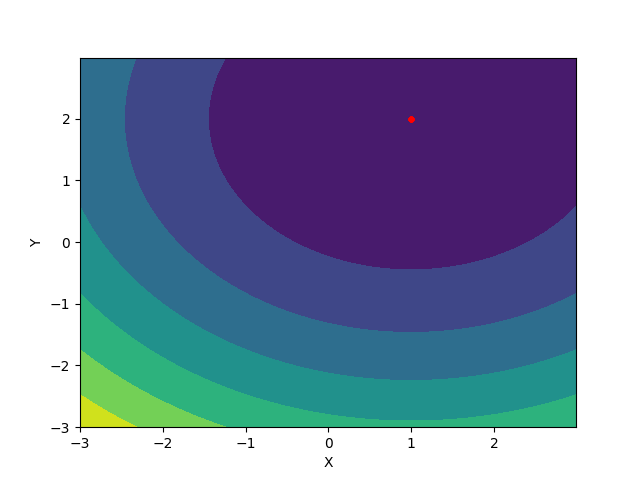
\includegraphics[scale=0.4]{imagens/translated_sphere/ses.png}}
\caption{Valores convergidos dos parâmetros para maximização da função para o caso da função matemática.}
\label{translated_sphere/ses}
\end{figure}

\begin{figure}[htbp]
\centering
\centerline{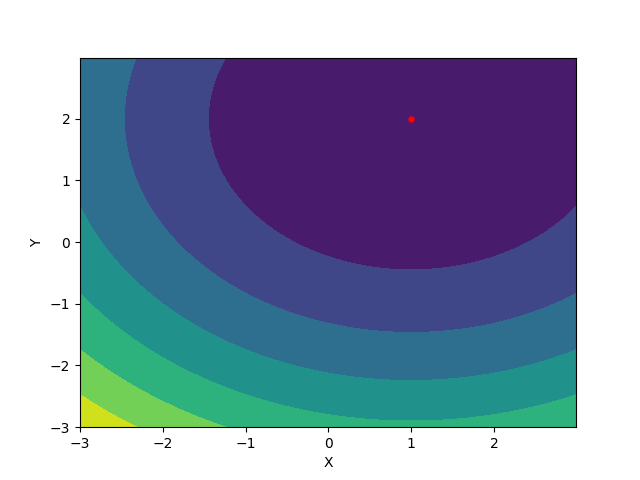
\includegraphics[scale=0.4]{imagens/translated_sphere/cmaes.png}}
\caption{Valores convergidos dos parâmetros para maximização da função para o caso da função matemática.}
\label{translated_sphere/cmaes}
\end{figure}

\begin{figure}[htbp]
\centering
\centerline{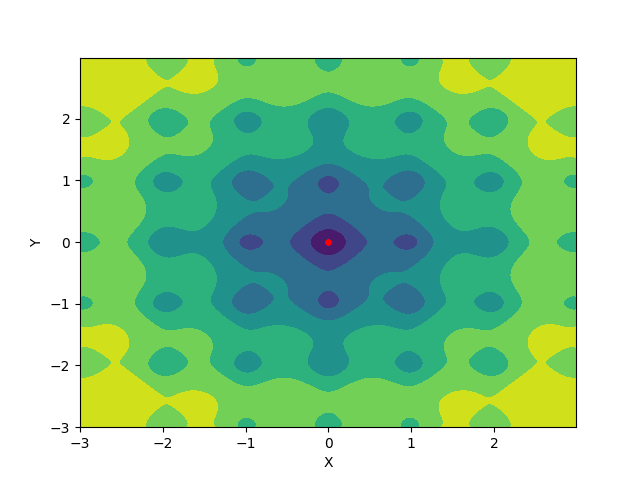
\includegraphics[scale=0.4]{imagens/ackley/ses.png}}
\caption{Convergência do valor da função qualidade com o passar das iterações para o caso da função matemática.}
\label{ackley/ses}
\end{figure} 

\begin{figure}[htbp]
\centering
\centerline{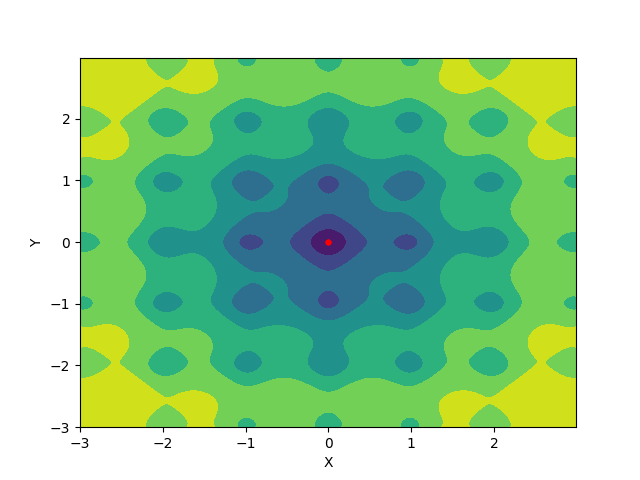
\includegraphics[scale=0.4]{imagens/ackley/cmaes.png}}
\caption{Convergência do melhor valor da função qualidade encontrado com o passar das iterações para o caso da função matemática.}
\label{ackley/cmaes}
\end{figure}

\subsection{Robô seguidor de linha}

Tendo em vista o correto funcionamento do algoritmo PSO dado o apresentado na subseção anterior e o comportamento coerente realizado pelo robô apresentado na Figura \ref{line_follower_solution}, pode-se concluir que os resultados apresentados na Figura \ref{line_parameters_convergence} são parâmetros satisfatórios do problema, chegando a convergência maximizada da Figura \ref{line_best_convergence}. Esses valores de parâmetros foram encontrados após cerca de 3000 iterações, levando a um valor de função qualidade máximo de 572.33; parâmetros esses: a velocidade linear do robô (0.72) e os ganhos proporcional, integrativo e derivativo (131.73, 624.82, 15.37, respectivamente).

\begin{figure}[htbp]
\centering
\centerline{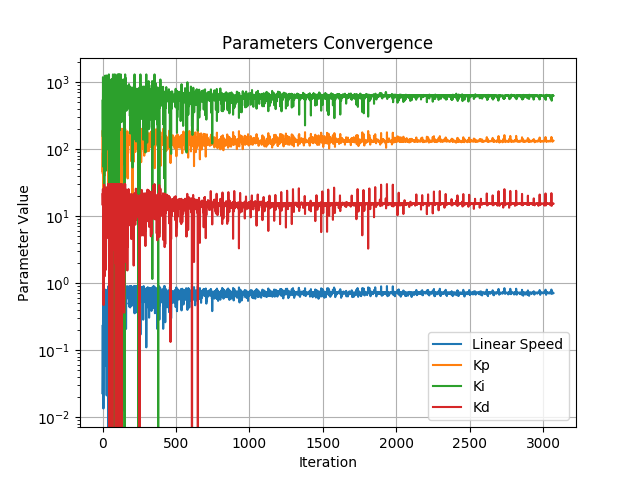
\includegraphics[scale=0.4]{line_parameters_convergence.png}}
\caption{Valores convergidos dos parâmetros para maximização da função para o caso do robô seguidor de linha.}
\label{line_parameters_convergence}
\end{figure}

\begin{figure}[htbp]
\centering
\centerline{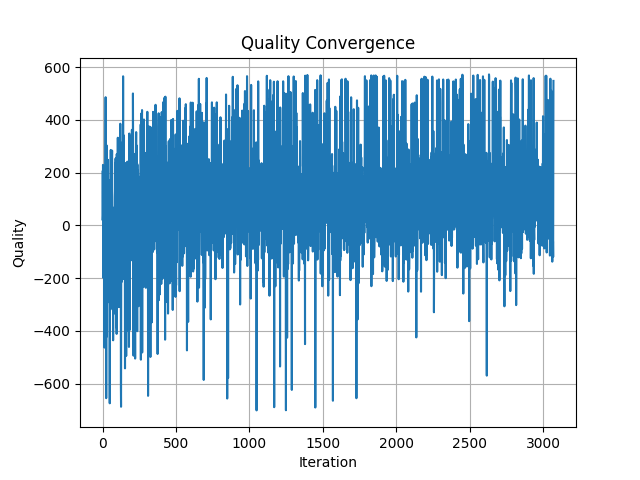
\includegraphics[scale=0.4]{line_quality_convergence.png}}
\caption{Convergência do valor da função qualidade com o passar das iterações para o caso do robô seguidor de linha.}
\label{line_quality_convergence}
\end{figure}

\begin{figure}[htbp]
\centering
\centerline{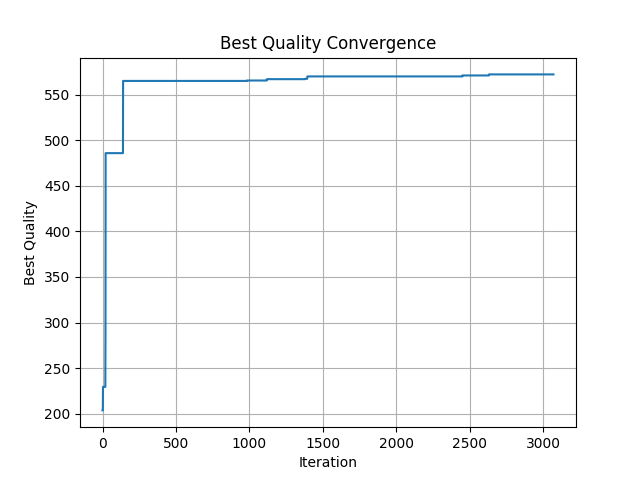
\includegraphics[scale=0.4]{line_best_convergence.png}}
\caption{Convergência do melhor valor da função qualidade encontrado com o passar das iterações para o caso do robô seguidor de linha.}
\label{line_best_convergence}
\end{figure}

\begin{figure}[htbp]
\centering
\centerline{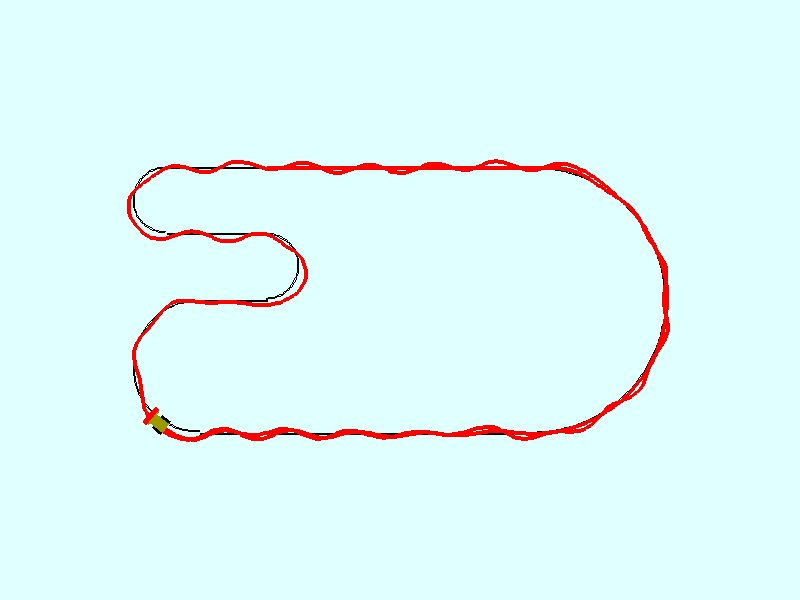
\includegraphics[scale=0.3]{line_follower_solution.jpeg}}
\caption{Simulação do robô seguidor de linha realizando o percurso com os valores de parâmetros encontrados a partir da otimização por PSO.}
\label{line_follower_solution}
\end{figure}

Tendo em vista o que foi apresentado, pode-se notar, por fim, que esse algoritmo realmente se demonstrou eficaz em encontrar parâmetros otimizados para uma determinada função de custo e um conjunto de possíveis soluções iniciais.

\begin{thebibliography}{00}
\bibitem{b1} M. Maximo, ``Roteiro: Laboratório 4 - Otimização com Métodos Baseados em População''. Instituto Tecnológico de Aeronáutica, Departamento de Computação. CT-213, 2019.
\end{thebibliography}

\end{document}
